\documentclass[11pt, a4paper]{article}

\usepackage[utf8]{inputenc}
\usepackage{graphicx}
\usepackage{hyperref}

\title{The End of Reactive Control: Algorithmic Certainty through Accounting and Audit by Design (A\&AD)}
\author{Richard G. Gasca Buelvas\thanks{Profesor de Cátedra de la Facultad de Ciencias Económicas y Administrativas, Pontificia Universidad Javeriana. Correo electrónico: co.auditoria@proton.me. Disclaimer: Las opiniones, análisis y conclusiones expresadas en este artículo son de exclusiva responsabilidad del autor y no comprometen ni representan la posición oficial de la Pontificia Universidad Javeriana. / The views, analyses, and conclusions expressed in this paper are solely those of the author and do not compromise, represent, or commit the Pontificia Universidad Javeriana.} \\ Pontificia Universidad Javeriana}
\date{June 2026}

\begin{document}

\maketitle

\begin{abstract}
Current frameworks of corporate governance and internal control are based on an unsustainable operational assumption: that accounting errors and discrepancies are inevitable. For decades, companies have depended on isolated databases and retrospective relational ledgers that treat data desynchronization, failures in financial reporting, and fraudulent activities as acceptable transactional frictions. Under this traditional paradigm, auditors and financial teams operate primarily as forensic investigators, relying on post-facto statistical sampling, long after capital has been allocated and risks have materialized. The resulting reconciliation debt drains corporate resources, reduces strategic flexibility, and clouds the visibility of boards of directors.

To resolve these inefficiencies, this article introduces the Accounting and Audit by Design (A\&AD) framework. The A\&AD model replaces retroactive verification with real-time deterministic assurance. By extending the shift-left paradigm to organizational control, A\&AD enforces regulatory compliance and fiscal constraints directly at the moment of economic origin: the initial contract or business event. By representing transactions as autonomous and immutable holons within semantic knowledge graphs, leveraging W3C standards such as JSON-LD and SHACL, internal control ceases to be a manual human intervention to become an intrinsic topological property of the data architecture itself. This approach systematically eliminates subsequent reconciliations, validates regulatory compliance at the exact point of data ingestion, and enables continuous auditing over the entirety of business events. Consequently, this model shifts the paradigm from simple data processing toward a rule-driven architecture, where system trust is designed directly into the data lifecycle, instead of being verified retrospectively.
\end{abstract}

\section{Introduction \& The Reconciliation Debt}

Since the historical codification of double-entry bookkeeping, the core architecture of corporate accounting has retained a fundamentally retrospective nature. Although the digitization of paper-based systems into relational Enterprise Resource Planning (ERP) databases modernized the recording medium, it did not resolve a critical structural deficiency: financial records remain static, flat logs of economic transactions that are completely detached from their underlying legal contracts and operational triggers. This disconnect---the "operational-regulatory seam"---constitutes a systemic vulnerability in modern business architectures, which organizations attempt to mitigate using constant, resource-heavy reconciliation protocols.

In the current era of rapid technological change, where corporations are deploying agentic Artificial Intelligence (AI) and autonomous software agents to execute core business processes, this reconciliation debt transforms from an administrative burden into a severe structural threat. Autonomous AI agents are now capable of independently executing supply chain agreements, purchasing resources, and finalizing contracts. Relational databases, however, lack the semantic expressiveness and multi-dimensional lineage tracking needed to audit these decentralized decisions. When an autonomous system initiates a transaction, current ERPs register the ledger adjustment but discard the complex decision-making context. This leaves oversight bodies and human auditors with opaque, "black-box" accounting outputs.

Cultivating trust within these AI-augmented corporate environments requires a complete shift in methodology: replacing retrospective statistical validation with absolute, deterministic correctness. Relying on statistical sampling for corporate governance is equivalent to structured guesswork---a compromise that no modern board of directors should accept.

This paper addresses this issue by proposing a "Moment 0" Semantic Digital Twin developed through Design Science Research (DSR). We argue that by shifting validation "left"---validating data integrity at the exact moment of transaction genesis---we can systematically prevent reconciliation discrepancies. Our proposed architecture integrates the Resource-Event-Agent (REA) framework with Semantic Web standards, decoupling the semantic meaning of economic events (using JSON-LD and XBRL GL) from specific software applications.

In addition, we introduce the use of hybrid "DataBooks" \cite{cagle2026} to serve as a standardized transport mechanism. By embedding structured Simple Knowledge Organization System (SKOS) taxonomies \cite{w3cskos2009} directly within the native training or system prompts of Large Language Models (LLMs), these DataBooks enable immediate, zero-shot auditing of business events by both human managers and autonomous oversight agents. The rest of this article outlines our theoretical foundations, describes the system architecture of the A\&AD Semantic Twin, and demonstrates an automated, real-time audit of an initial equity distribution.

\section{Related Work \& Theoretical Framework}

The theoretical foundation of the A\&AD architecture lies at the intersection of the Zachman Enterprise Architecture Framework, Tim Berners-Lee's Semantic Web Stack \cite{bernerslee2001}, ontological accounting frameworks, and the audit capabilities of modern generative artificial intelligence. This integration leverages Zachman's structured classification to map organizational questions (What, How, Where, Who, When, Why) directly onto the technical layers of Berners-Lee's Semantic Web Stack---spanning from RDF/OWL representations to rules, cryptographic proofs, and systemic trust layers---aiming to heal the historic division that separates operational business logic from financial ledger records.

\subsection{The REA Paradigm and Graph-Based Digital Twins}
The conceptual origins of this events-based paradigm trace back to George H. Sorter (1969) \cite{sorter1969}, who proposed an "events approach" to accounting theory. Sorter argued that accounting systems should record and compile detailed data of individual economic events, allowing users to generate customized reports from this raw information rather than relying solely on traditional aggregated financial summaries. This paradigm is further reinforced by Shyam Sunder's (1997) theory of accounting and control \cite{sunder1997}, which conceptualizes the firm as a nexus of contracts. Under Sunder's view, a corporate entity is a sum of contracts among resource providers, where the role of accounting is to monitor and enforce these agreements. A\&AD operationalizes this theory by representing each contract independently within the semantic knowledge graph as an autonomous node with all its attributes. Consequently, the graph directly tracks economic transactions (events) alongside the corresponding sources and uses of resources. McCarthy (1982) \cite{mccarthy1982} subsequently formalized these events-based concepts into the Resource-Event-Agent (REA) accounting framework, which argues that accounting records must reflect the economic substance of transactions rather than just their accounting artifacts. The REA model focuses on the fundamental nature of economic events: the participants (Agents), the values traded (Resources), and the transactions themselves (Events). Subsequent researchers (e.g., Fischer-Pauzenberger \& Schwaiger, 2017 \cite{fischer2017}) have formalized REA into a rigorous ontology (OntoREA) using foundational frameworks like the Unified Foundational Ontology (UFO). Furthermore, OntoREA has been extended to model dynamic hedge portfolios for financial derivatives \cite{fischer2018}. While these developments demonstrate REA's capability in representing complex financial instruments using custom ontologies, our A\&AD framework approaches the representation of legal entities and financial agreements by directly integrating industry-standard ontologies, such as the Financial Industry Business Ontology (FIBO) \cite{fibo2020} and the Algorithmic Contract Types Unified Standards (ACTUS) \cite{actus2018}, within the transactional graph. Crucially, A\&AD changes the data pipeline topology: rather than routing transactions through a relational ERP to be later converted into a graph, the contract genesis at Moment 0 is represented in XBRL GL and immediately transmuted into a JSON-LD payload to be injected directly into the semantic knowledge graph. Traditional bookkeeping registers can run in parallel. In a secondary phase, legacy systems can be synchronized and updated by querying the semantic graph, preserving legacy structures without compromise to the integrity of transaction genesis. Regardless of the specific ontological approach, deploying these designs in a practical, scaleable environment requires transitioning away from traditional relational database engines toward Semantic Knowledge Graphs. Graph databases are uniquely suited to preserving complex, multi-dimensional connections without the constraints of rigid schemas.

\subsection{Model-Driven Systems, XBRL GL, and Supply Chain Integration}
The boundary between business operations and external reporting is directly addressed by Hoffman's "Model-Driven Enterprise Architecture" \cite{hoffman2025}. Hoffman argues for replacing disjointed, proprietary data silos with unified, standardized reporting pipelines. The Extensible Business Reporting Language Global Ledger (XBRL GL) plays a vital role in this design. While XBRL FR (Financial Reporting) is designed for end-of-period aggregations, XBRL GL captures and standardizes low-level transactional details. Within this standard, the use of the \texttt{accountingPurposeCode} element is crucial, as it allows for the explicit classification and tagging of the purpose of each accounting entry or record (such as IFRS, US GAAP, local standards, or tax purposes) from the genesis of the data. By mapping and transmuting this tag to the semantic graph, the classic challenge of coexisting reporting frameworks is resolved: the same transactional event can be dynamically queried and filtered according to its purpose using graph query languages, ensuring full granularity and eliminating record duplication in parallel ledgers. Implementing XBRL GL as a core data format allows companies to establish platform-independent interoperability. This ensures that audit trail data travels from operational genesis (Moment 0) to regulatory endpoints without loss of semantic meaning.

This integration expands upon the foundational vision of the W3C (2009) regarding the convergence of XBRL and the Semantic Web. By extending the transactional capabilities of XBRL Global Ledger (XBRL GL) to encompass the broader lifecycle of the supply chain (from event triggering to final invoice), A\&AD captures both quantitative financial information and operational non-financial data. This comprehensive consolidation within the semantic graph enables the direct generation of both traditional financial reports (such as the statement of financial position and performance reports) and corporate sustainability (ESG) and supply chain reports without requiring additional extraction and re-mapping processes. To govern this multi-dimensional flow, the framework incorporates the Zachman Enterprise Architecture Framework, utilizing its structured rows and columns to map operational actions directly onto the technical layers of the semantic stack.

\subsection{Explainable AI, SKOS Structuring, and DataBooks}
As machine learning models are tasked with financial auditing, mitigating the risk of artificial intelligence "hallucinations" becomes paramount. Cagle and Shannon \cite{cagle2026} introduce "DataBooks" as a bridging format: hybrid Markdown files containing embedded, machine-readable JSON-LD payloads. DataBooks effectively connect narrative texts (such as legal agreements) with structured machine data (semantic graphs).

Furthermore, embedding Simple Knowledge Organization System (SKOS) taxonomies directly into LLM architectures represents a major advance for "Explainable AI." As Cagle and Shannon \cite{cagle2026} note, standard ontologies perform significantly better when integrated directly into the LLM compilation phase. Instead of loading complex, multi-volume regulatory rules (e.g., IFRS or US GAAP) into an LLM's temporary context window---which is computationally inefficient and increases error rates---the AI auditor can leverage the model's pre-existing knowledge of standardized SKOS structures. The individual DataBook only needs to supply the specific, localized concepts relevant to the transaction. This combination allows AI auditing agents to evaluate complex graphs with high precision, bound by clear ontological boundaries, thereby facilitating continuous, independent monitoring.

\section{Artifact Design: The A\&AD Semantic Digital Twin}

Consistent with Design Science Research principles, our primary contribution is the design and implementation of a Semantic Digital Twin. This artifact is built to span the operational-regulatory gap by creating a continuous, verifiable data pipeline from inception to reporting. The architecture comprises a conceptual blueprint and three distinct physical layers: the Conceptual Navigational Matrix, the Operational Graph Engine, the Semantic Transmutation Layer, and the Living Knowledge Wrapper.

\subsection{The Conceptual Blueprint: The A\&AD Navigational Matrix}
Before detailing the physical implementation, the A\&AD framework establishes a conceptual blueprint represented by the A\&AD Reference Atlas. This artifact fuses the Zachman Framework columns (Why, How, What, Who, Where, When) with the W3C Semantic Web stack. The resulting matrix acts as a navigational map, mapping business motivations and operational events to graph assets and cryptographic validations. This interactive schema, deployed at \url{https://ai2accountans.github.io/AAbD/}, coordinates the engineering layers and ensures that any data asset preserves its operational and regulatory meaning as it traverses the stack.

\begin{figure}[htbp]
    \centering
    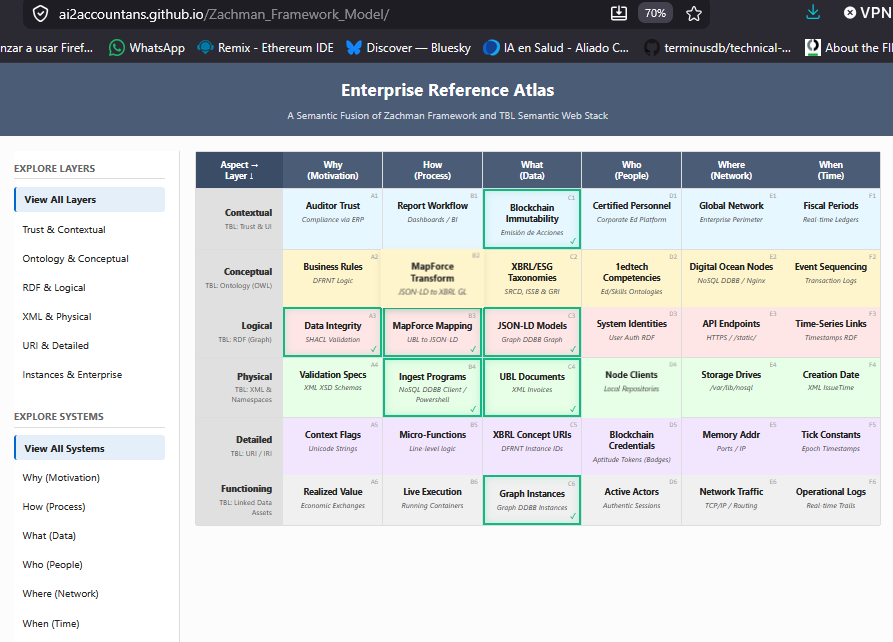
\includegraphics[width=\textwidth]{aad-zachman-atlas.png}
    \caption{The A\&AD Reference Atlas: Fusing Zachman Framework and W3C Semantic Web Layers.}
    \label{fig:aad_atlas}
\end{figure}

\subsection{The Operational Graph Engine (TerminusDB \& DFRNT)}
At the bottom of the system stack, relational database engines are replaced by TerminusDB, a native RDF/OWL graph database. This graph layout enables the enterprise to represent the core dimensions of the Zachman Framework (specifically Agents, Resources, Events, and Locations) as interconnected nodes and relationships instead of dispersed tables. To query and manage this operational graph, our design employs the DFRNT semantic data platform. Through QOWL (GraphQL over OWL), monitoring agents can retrieve targeted transactional sub-graphs. This query process focuses on the exact moment of transaction genesis---the "Moment 0"---collecting not only currency figures, but the complete operational lineage of all participating agents and assets.

\subsection{The Semantic Transmutation Layer (Altova XMLSpy \& MapForce)}
Raw JSON data retrieved from the operational database frequently uses internal company terminology and lacks the standardized regulatory terminology required for audit verification. To address this difference without hardcoding translation rules, the architecture integrates the Altova product suite to handle semantic transmutation. First, Altova XMLSpy serves as the schema design workspace, used to define the JSON-LD schemas and enforce W3C SHACL (Shapes Constraint Language) constraints. This guarantees that the core ontology is logically valid prior to data processing.

Following schema validation, Altova MapForce serves as a format-neutral data mapper. It parses the raw JSON payload and applies the W3C and XBRL GL ontologies designed in XMLSpy. This automated mapping transforms the internal operational logs into a standardized JSON-LD graph instance. In traditional XBRL architecture, validations and business rules are implemented through the \emph{XBRL Formula Linkbase}. In the A\&AD framework, upon transmuting the XBRL GL instances into the semantic graph, this control logic is mapped and executed using the W3C \textbf{SHACL (Shapes Constraint Language)} standard. SHACL allows for the definition of structural and mathematical integrity constraints (such as verifying that the sum of debits matches credits in a transaction, or enforcing share issuance limits) directly over the nodes and relationships of the graph. This layered architecture ensures that double-entry balance and structural compliance are verified before the data is exposed for external review, shifting accounting control rules from a post-facto phase to preventative real-time control at the exact moment of data ingestion. This configuration is empirically validated by historical industry precedents, such as the Maryland Association of CPAs (MACPA) case study \cite{altova_macpa}, which proved the viability of using Altova's design suite (XMLSpy and MapForce) to translate heterogeneous ledger databases into standardized XBRL GL structures.

\subsection{The Living Knowledge Wrapper (DataBooks)}
The final phase of the A\&AD data pipeline handles the interaction between human users and automated systems. The structured JSON-LD output is packaged into a "DataBook"---a hybrid Markdown document. The DataBook combines a human-readable narrative (such as a corporate charter or partnership agreement) with hidden, machine-readable JSON-LD data segments. This document serves as a self-contained, unchangeable "holon." Human supervisors can review the business context in plain text, while autonomous AI agents can parse the embedded graph data using pre-trained SKOS taxonomies. This decoupled design provides high certainty without requiring the AI to process raw, unstructured language, completing the "Shift-Left" audit process.

\section{Demonstration: The Genesis Moment Case Study}
To validate the A\&AD framework, a practical Proof of Concept (PoC) was executed modeling the "Moment 0" of a corporate entity. The origin of the entity is an agreement of wills among the founding partners, captured in an official document elevated to a public deed in a notary's office (represented by the file \texttt{SOCIEDAD\_LIMITADA.pdf} located in the incorporation deed directory). From this legal document, the terms and data of the agreement are extracted and enriched with accounting semantics (manually, for illustrative purposes of this demonstration) to prepare the dataset to begin its journey through the semantic pipeline.

\subsection{Genesis Data Extraction}
The terms and capital contributions of the corporate agreement (the partners, their equity shares, and tax identifiers) were structured in a tabular format within a Google Sheet (publicly available for audit at \url{https://docs.google.com/spreadsheets/d/1SzBin5R74djTxuyLG_9AMUpOf_Uwwo9J5bE4HHykiAM/edit?usp=sharing}) to serve as the operational starting point of the data pipeline. These raw data are exported in CSV format representing the initial ledger entry, prepared to begin their transmutation to the standard XBRL GL taxonomy without traversing a traditional relational Enterprise Resource Planning (ERP) database.

\subsection{Semantic Transmutation}
This raw CSV source file was loaded into Altova MapForce. We created a visual data mapping structure to align the internal ledger structure with the XBRL GL taxonomy. During this process, local fields were mapped to standardized semantic elements, including \texttt{gl-cor:amount}, \texttt{gl-cor:measurableQuantity}, and \texttt{gl-cor:accountMainID}. Altova MapForce processed the input to generate a standardized JSON-LD graph instance of the transaction, successfully translating internal nomenclature into the universal XBRL GL taxonomy.


\subsection{Ingestion and Querying in DFRNT / TerminusDB}
The semantic integration and query phase represents the operational culmination of our pipeline, where the JSON-LD graph acquires logical meaning within the DFRNT ecosystem (which hosts the TerminusDB database). This process consists of five sequential steps:
\begin{enumerate}
    \item \textbf{Class and Ontology Definition (Step 1):} First, semantic classes and schemas are structured within the DFRNT interface. Core accounting entities (such as \texttt{EntryDetail} and \texttt{GistPerson}) are defined, mapping them to industry-standard ontologies (FIBO, ACTUS, and gist) to ensure typological and legal consistency (see Fig.~\ref{fig:dfrnt-step1}).
    \item \textbf{JSON-LD Payload Ingestion (Step 2):} Once the schema is defined, the transmutated JSON-LD instance is injected directly via DFRNT's ingestion console. This payload is stored immutably under TerminusDB's closed-world constraints (see Fig.~\ref{fig:dfrnt-step2}).
    \item \textbf{Logical Digital Twin Visualization (Step 3):} With the data loaded, DFRNT's Graph Data Browser enables visual exploration of the resulting graph. This represents the "Logical Twin" of the enterprise at Moment 0, showing how each partner (\texttt{GistPerson}) is linked to their respective transactional line (\texttt{EntryDetail}) (see Fig.~\ref{fig:dfrnt-step3}).
    \item \textbf{GraphQL/QOWL Query Construction and Execution (Step 4):} To verify that relations and balances remain intact, a GraphQL-over-OWL (QOWL) query named \texttt{AccionesYValorPorSocio} is executed in DFRNT, filtering the \texttt{EntryDetail} class to extract the amount, partner identifier, and share quantity (see Fig.~\ref{fig:dfrnt-step4}).
    \item \textbf{Query Results Analysis (Step 5):} Finally, DFRNT displays the query results in a structured JSON response, confirming the exact contributions (e.g., Founding Partner A with 2,500,000 COP and 2,500 shares), proving data integrity across the transformations (see Fig.~\ref{fig:dfrnt-step5}).
\end{enumerate}

\begin{figure}[htbp]
    \centering
    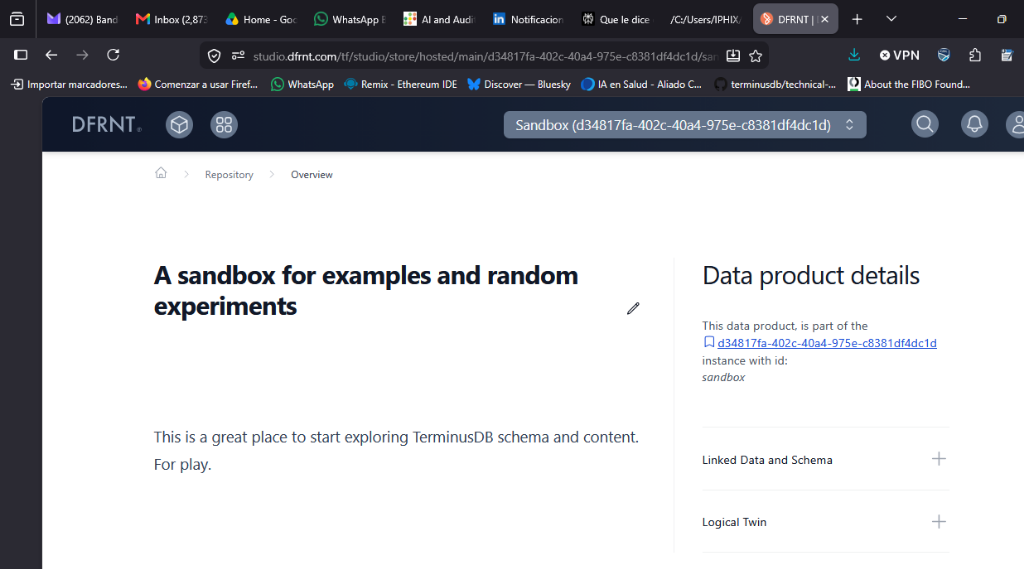
\includegraphics[width=0.9\textwidth]{dfrnt-step1.png}
    \caption{DFRNT Class and Ontology Definition.}
    \label{fig:dfrnt-step1}
\end{figure}

\begin{figure}[htbp]
    \centering
    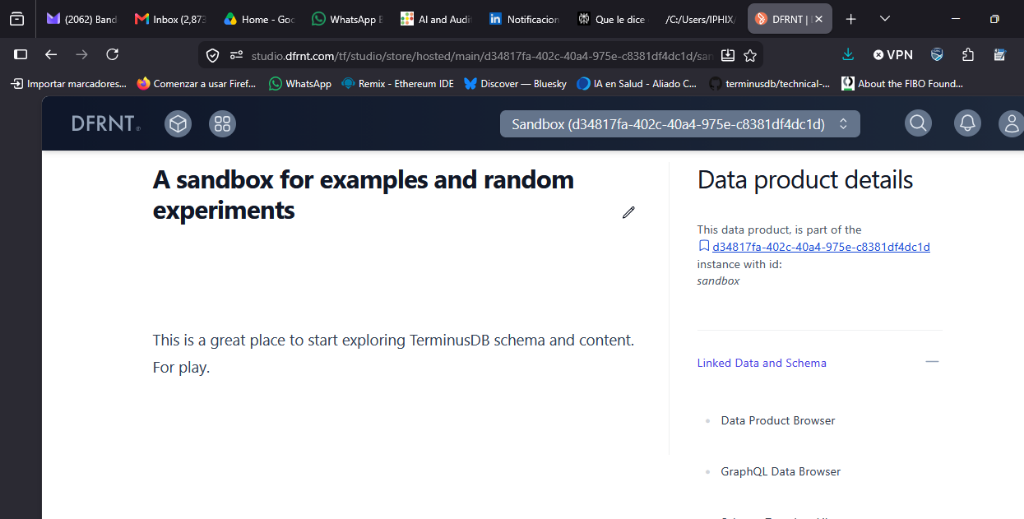
\includegraphics[width=0.9\textwidth]{dfrnt-step2.png}
    \caption{JSON-LD Ingestion Console in DFRNT.}
    \label{fig:dfrnt-step2}
\end{figure}

\begin{figure}[htbp]
    \centering
    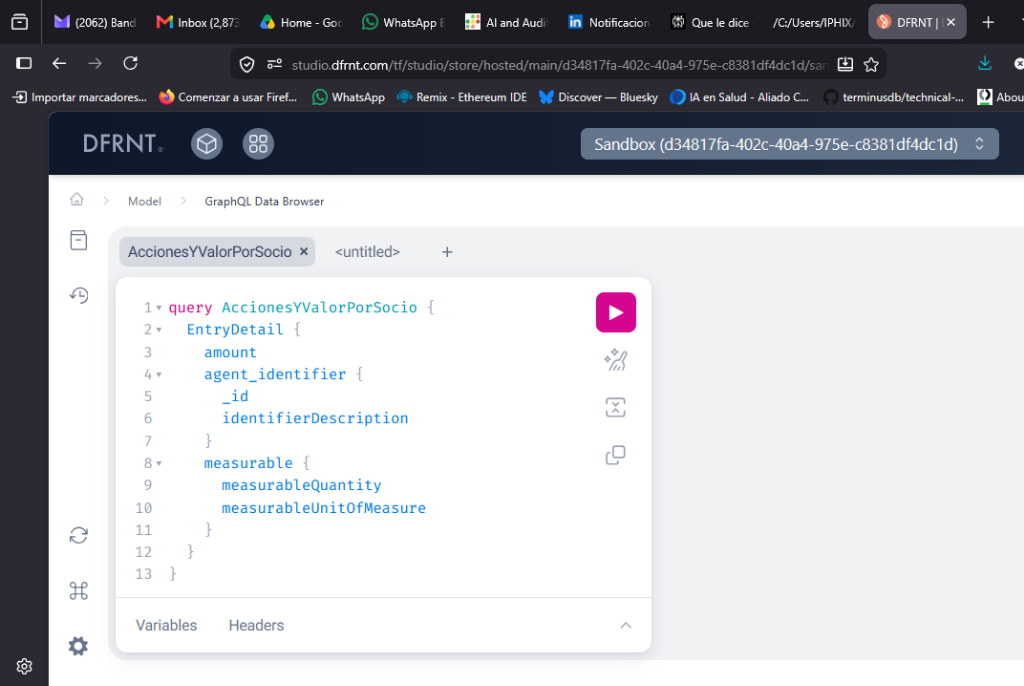
\includegraphics[width=0.9\textwidth]{dfrnt-step3.png}
    \caption{DFRNT Graph Visualizer - Logical Twin at Moment 0.}
    \label{fig:dfrnt-step3}
\end{figure}

\begin{figure}[htbp]
    \centering
    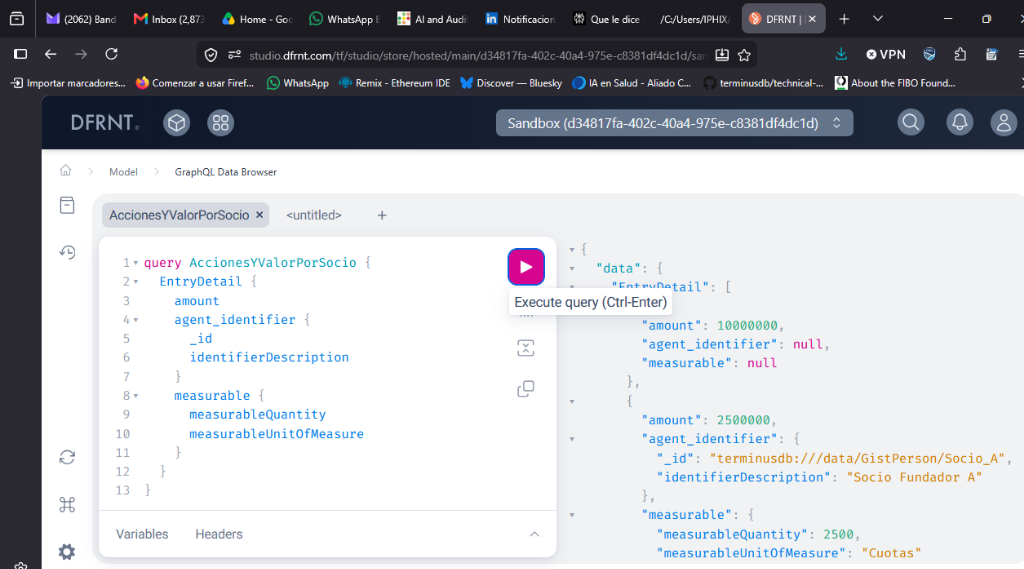
\includegraphics[width=0.9\textwidth]{dfrnt-step4.png}
    \caption{GraphQL / QOWL Query Construction in DFRNT.}
    \label{fig:dfrnt-step4}
\end{figure}

\begin{figure}[htbp]
    \centering
    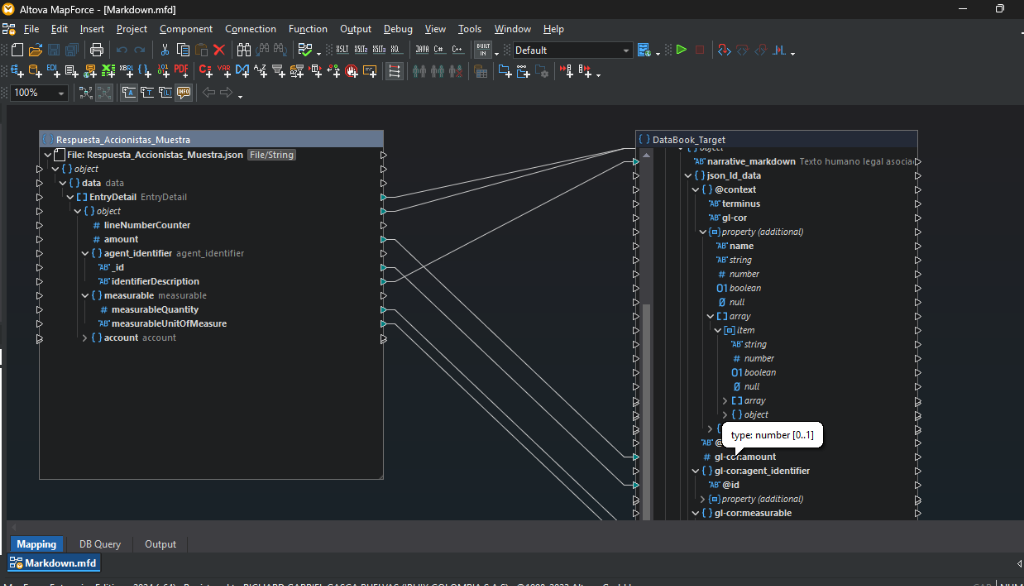
\includegraphics[width=0.9\textwidth]{dfrnt-step5.png}
    \caption{GraphQL Query Results in DFRNT.}
    \label{fig:dfrnt-step5}
\end{figure}

\subsection{Autonomous Audit Execution}
The output of the Altova MapForce mapping is consolidated into a hybrid Markdown file named \texttt{output.databook.md}, which constitutes the target DataBook. This file establishes a dual-purpose record combining the natural language incorporation deed with the underlying JSON-LD transactional graph. To test automated verification independently and externally to the operational database, auditing tests were executed on this file within a Google Colab environment using the notebook \texttt{MarkDown\_1.ipynb} (stored locally in \texttt{C:\textbackslash{}Users\textbackslash{}IPHIX\textbackslash{}Documents\textbackslash{}Projects\textbackslash{}DFRNT\textbackslash{}Momento0\textbackslash{}Google Colab\textbackslash{}}).

The automated audit workflow, constructed in Jupyter Notebook cells and executed using Python's \texttt{rdflib} library, consists of the following detailed steps:
\begin{enumerate}
    \item \textbf{Environment Preparation (Step 0):} First, Google Colab is connected to Google Drive using \texttt{drive.mount('/content/drive')} to access the file path of \texttt{output.databook.md}. Next, the Python semantic web library \texttt{rdflib} is installed silently (\texttt{!pip install rdflib -q}), and the necessary \texttt{Graph} and \texttt{json} modules are imported (see Fig.~\ref{fig:colab-step1}).
    \item \textbf{Reading the DataBook (Step 1):} The hybrid Markdown file is opened and its entire contents are read from the specified Google Drive path (see Fig.~\ref{fig:colab-step1}).
    \item \textbf{JSON-LD Blocks Extraction (Step 2):} Using straightforward string parsing techniques, the script splits the file using the code block delimiter \texttt{```json-ld} to isolate and extract the embeddable JSON-LD graph segments (see Fig.~\ref{fig:colab-step1}).
    \item \textbf{Semantic Graph Loading and Compilation (Step 3):} An RDFLib \texttt{Graph()} object is initialized in memory, and the extracted JSON-LD data blocks are iterated over. Using the function \texttt{g.parse(data=b, format='json-ld')}, the data is parsed to locally compile the semantic accounting graph (see Fig.~\ref{fig:colab-step2}).
    \item \textbf{SPARQL Mathematical Auditing and Verification (Step 4):} A declarative SPARQL query is executed over the graph, which defines the XBRL GL taxonomy prefix (\texttt{PREFIX gl-cor: <http://www.xbrl.org/int/gl/cor/2015-03-25\#>}) and sums all atomic transactional amounts associated with the \texttt{gl-cor:amount} property. As shown in the console printout results, the audit script successfully computes and prints a verified total capital amount of \texttt{\$10,000,000 COP} (see Fig.~\ref{fig:colab-step2}).
\end{enumerate}

\begin{figure}[htbp]
    \centering
    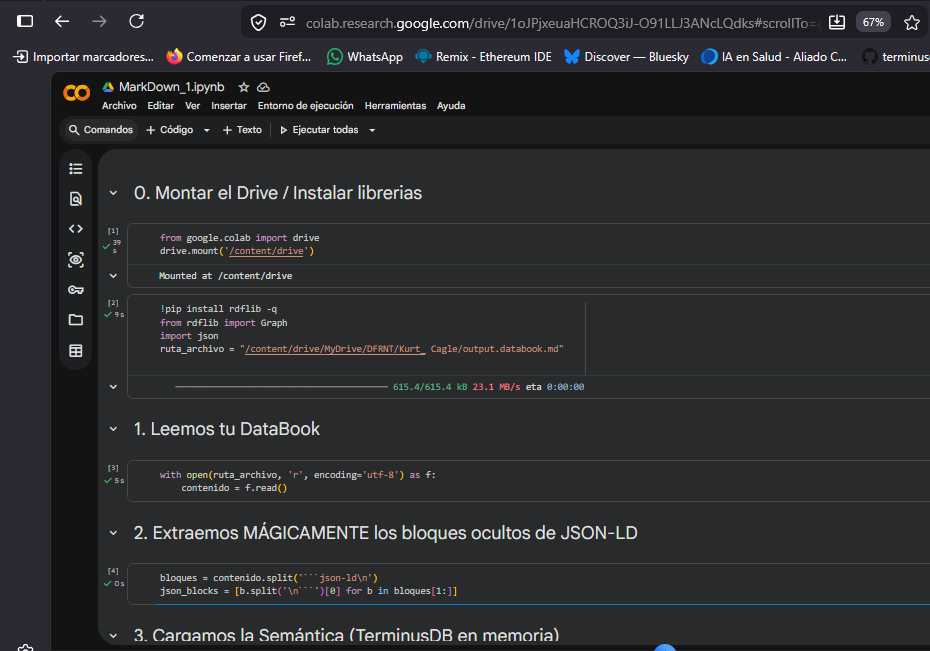
\includegraphics[width=0.9\textwidth]{colab-step1.png}
    \caption{Jupyter Notebook Environment Setup and DataBook Parsing.}
    \label{fig:colab-step1}
\end{figure}

\begin{figure}[htbp]
    \centering
    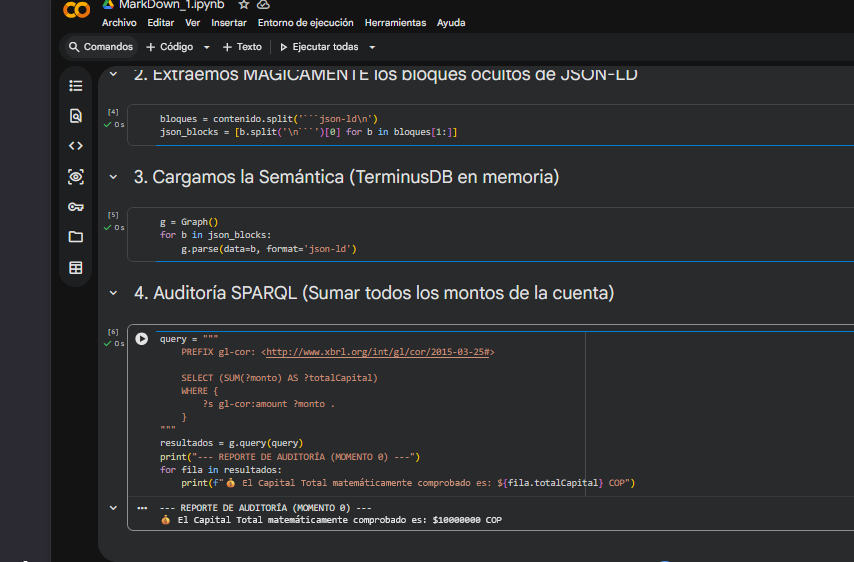
\includegraphics[width=0.9\textwidth]{colab-step2.png}
    \caption{In-memory Semantic Graph Ingestion and SPARQL Query execution.}
    \label{fig:colab-step2}
\end{figure}

The script successfully computed the exact sum of the founding capital, demonstrating that a machine---independent of the original operational database and reading only the \texttt{output.databook.md} file---could parse a text document, extract the foundational taxonomy, and mathematically prove the financial position with absolute certainty.

\section{Conclusion}

A reliance on retrospective reconciliation processes is an outdated habit of the relational database age. As shown by the Accounting and Audit by Design (A\&AD) model, moving verification procedures "left" to the moment of data creation is both conceptually sound and technically achievable. By integrating the REA ontology, TerminusDB knowledge graphs, and hybrid DataBooks, organizations can package economic activities into self-contained, self-verifying semantic records.

From the analysis and implementation of this architecture, three key conclusions emerge regarding the benefits of the A\&AD framework:
\begin{enumerate}
    \item \textbf{Definitive Eradication of Reconciliation Debt through "Accounting Shift-Left":} By capturing and validating the transactional semantics and context at "Moment 0" (the origin of the economic event), A\&AD eliminates the need for complex, retrospective reconciliations. Resolving data inconsistency at the point of ingestion removes the reliance on manual spreadsheets for late-stage adjustments, enabling a real-time, friction-free business view.
    \item \textbf{Internal Control as a Topological Property of the Graph (SHACL):} Instead of relying on static policy manuals and regulatory limits verified forensically or manually, A\&AD moves governance and compliance rules into hard logical constraints at the database level using SHACL (Shapes Constraint Language). Double-entry balance, authorized signatures, and transaction thresholds become intrinsic, unbreakable properties of the data structure, preventing corrupt records from being written.
    \item \textbf{Explainable Governance and Deterministic Auditing for the Agentic AI Era:} A\&AD provides the trust infrastructure required to oversee both human transactions and autonomous decisions executed by AI software agents. Through hybrid DataBooks (Markdown + JSON-LD) and deterministic SPARQL queries on in-memory knowledge graphs, the system enables immediate, high-fidelity, "zero-shot" auditing. This completely eliminates the risk of LLM hallucinations during compliance tasks by binding the AI to formal ontological boundaries.
\end{enumerate}

Our future work will focus on extending this proof of concept to handle ongoing operational transactions and deploying real-time SHACL validation guards at the database level, laying the groundwork for automated, model-driven corporate governance.

\begin{thebibliography}{99}

\bibitem{actus2018}
ACTUS Financial Research Foundation. (2018).
\emph{Algorithmic Contract Types Unified Standards (ACTUS)}.
Retrieved from \url{https://www.actusfrf.org/}.

\bibitem{bernerslee2001}
Berners-Lee, T., Hendler, J., \& Lassila, O. (2001).
The Semantic Web.
\emph{Scientific American}, 284(5), 34--43.

\bibitem{cagle2026}
Cagle, K., \& Shannon, C. (2026).
\emph{DataBook Pipelines: From Raw Data to Living Knowledge}.
The Ontologist.
Retrieved from \url{https://ontologist.substack.com/p/databook-pipelines}.

\bibitem{altova_macpa}
Altova. (2010).
\emph{Case Study: Maryland Association of CPAs (MACPA) Integrates Accounting Systems with XBRL GL and Altova MapForce}.
Retrieved from \url{https://www.altova.com/documents/macpa_casestudy.pdf}.

\bibitem{fibo2020}
EDMC. (2020).
\emph{Financial Industry Business Ontology (FIBO)}.
Enterprise Data Management Council.
Retrieved from \url{https://spec.edmcouncil.org/fibo/}.

\bibitem{fischer2017}
Fischer-Pauzenberger, C., \& Schwaiger, W. S. (2017).
OntoREA: A foundational ontology-based formalization of the REA accounting model.
\emph{Journal of Information Systems}, 31(3), 43--69.

\bibitem{fischer2018}
Fischer-Pauzenberger, C., \& Schwaiger, W. S. (2018).
OntoREA© Accounting and Finance Model: Hedge Portfolio Representation of Derivatives.
In \emph{IFIP Working Conference on The Practice of Enterprise Modeling} (pp. 372--382). Springer, Cham.
\url{https://doi.org/10.1007/978-3-030-02302-7_24}.

\bibitem{hoffman2025}
Hoffman, C. (2025).
\emph{Rethinking Financial Reporting: the Model-driven Financial Statement}.
Seattle Method.
Retrieved from \url{https://seattlemethod.blogspot.com/}.

\bibitem{mccarthy1982}
McCarthy, W. E. (1982).
The REA accounting model: A generalized framework for accounting systems in a shared data environment.
\emph{The Accounting Review}, 57(3), 554--578.

\bibitem{sorter1969}
Sorter, G. H. (1969).
An "events" approach to basic accounting theory.
\emph{The Accounting Review}, 44(1), 12--19.

\bibitem{sunder1997}
Sunder, S. (1997).
\emph{Theory of Accounting and Control}.
South-Western College Publishing.

\bibitem{w3c2009}
W3C. (2009a).
\emph{XBRL and the Semantic Web}.
W3C Interest Group Report.
Retrieved from \url{https://www.w3.org/2009/03/xbrl/old-report.html}.

\bibitem{w3cskos2009}
W3C. (2009b).
\emph{SKOS Simple Knowledge Organization System Reference}.
W3C Recommendation.
Retrieved from \url{https://www.w3.org/TR/skos-reference/}.

\end{thebibliography}

\end{document}
